\documentclass[a4paper]{article}

%% Useful packages
\usepackage{amsmath}
\usepackage{graphicx}
\usepackage[colorinlistoftodos]{todonotes}
\usepackage[colorlinks=true, allcolors=black]{hyperref}
\usepackage[fontsize=11pt]{scrextend}
\usepackage{titlesec}
 \usepackage[section]{placeins}

\setlength\parindent{0pt}
\titleformat*{\section}{\Large\bfseries}
\titleformat*{\subsection}{\Large\bfseries}

\title{PowerEnjoy Service - Design Document}

\begin{document}

\begin{titlepage}
\begin{figure}
\centering

\includegraphics[width=0.2\textwidth]{polimi.jpg}
\par
\LARGE Politecnico di Milano
\end{figure}


\maketitle
\textbf{Version 1.1}
\newline

\raggedright
Authors:
\begin{itemize}
	\item Domenico FAVARO (Mat. 837995)
        	\item Matheus FIM (Mat. 876069)
	\item Caio ZULIANI (Mat. 877266)	
\end{itemize}
\raggedleft
Prof. Elisabetta DI NITTO
\thispagestyle{empty}
\end{titlepage}

\tableofcontents
\newpage
 
\section{Introduction}
\subsection{Purpose}
This Design Document serves the purpose to present to all parties interested the description of the structure for the PowerEnjoy Service. It provides documentation of Software, Architecture and other important aspects of Design to help the understanding and development of the System. Every component that is implemented for the System will be explained as well as the purpose they serve to contribute to the fullfilment of all the project Requirements. All strategies and design decisions will be documented as well. Software Design Description, decisions and key information to be used to communicate the general purpose of the structure to our stakeholders, and serve as detailed documentation for the components of the System for the developers.

\subsection{Scope}
This Document presents the PowerEnjoy Service System, an electric car sharing service. To better understand the broader scope of the service, it is presented in the RASD Document. This Document will not include detailed information on all the tools and protocols that will be used in the development of the System but rather their purpose and functionality inside the PowerEnjoy System. As example, general knowledge of the Client-Server structure is expected as it will not be rigorously explained but instead how such structure will be used to satisfy our System's Requirements. 

\subsection{Glossary: Definitions, Acronyms, Abbreviations}
\begin{itemize}
\item \textbf{RASD:} Reqirements And Specifications Document.
\item \textbf{DD:} Design Document.
\item \textbf{Java EE:} Java Enterprise Edition. Software Development Platform.
\item \textbf{App:} Application. Refers to the deployed service as Web or Mobile Application.
\item \textbf{Component:} Software element that implements and offer functionalities in the System.
\item \textbf{EJB:} Enterprise Java Beans. Component in the Business Tier for the Application Logic.
\item \textbf{DBMS:} DataBase Management System.
\item \textbf{JDBC:} Java Database Connectivity, Java API to connect to DataBases.
\item \textbf{HTTPS:} Hypertext Transfer Protocol over TLS. Protocol to safefully communicate over the Internet.
\item \textbf{TLS:} Transport Layer Security that provides communication security.
\item \textbf{REST/RESTful:} Representational state transfer, architectural style for the System communications.
\item \textbf{API:} Application Programming Interface.
\end{itemize}
For other concepts concerning the Service definition look in the \textbf{Glossary} section of the RASD.

\subsection{Reference Documents}
\begin{itemize}
\item Specification Document: Assignments AA 2016-2017.pdf
\item PowerEnjoy Requirements And Specifications Document (RASD)
\item IEEE Std 1016-2009 IEEE Standard for Information Technology-Systems Designs-Software Design Descriptions (SDD IEEE 1016-2009.pdf)
\item Example Documents:
\begin{itemize}
\item[-] Sample Design Deliverable Discussed on Nov. 2.pdf
\item[-] Software Design Document (SDD) Template (sdd\_template.pdf)
\end{itemize}
\end{itemize}

\subsection{Document Structure}
\begin{description}
\item \textbf{Section 1 - Introduction:} This section provides a general description of the purpose and structure of this Design Document.
\item \textbf{Section 2 - Architectural Design:} This section illustrates a broader to specific view of the components that form part of the System, presenting from the overview of the architecture of the system to a description of how each component will interface inside the structure.
\item \textbf{Section 3 - Algorithm Design:} Important functionalities of the System that require the development of algorithms will be described in this section.  
\item \textbf{Section 4 - User Interface Design:} All details refering to how the User will interface with the System, from the Web Application to the screens inside the Cars will be shown in this section. As well as general mockups of the Graphical User Interface (GUI) screens.
\item \textbf{Section 5 - Requirements Traceability:} In this section is explained how the Design decisions and structure help fulfill the Requirements for the System that were defined in the RASD. 
\item \textbf{Section 6 - Effort Spent:} Detailed record of the hours worked for each member of the team is documented in this section.
\item \textbf{Section 7 - References:} Any reference to additional external sources that can help the better understanding of this Document is documented in this section.
\end{description}

\newpage
\section{Architectural Design}
\subsection{Overview}
As was show in the Proposed System part of the RASD, the PowerEnjoy structure will consist on a 3-tier Client-Server Architecture. The server part built on a JEE Platform with access to the Company's Database Server and the Client consisting of Users, CRM and Cars that will use a browser to access our Web Application and a Mobile Device and Screen inside the Cars will access the Mobile Application.
As we need to interface our application with the Car functions (i.e. Lock, Unlock, Battery state) the application must have some Logic implemented client side. This distributed Logic structure will allow GUI to be created on the Client side as well.
The Database Server will belong to the Company and will allow registration of User, Reservations, Rides and Payments. Cars, CRM Employees and Parking Locations are asumed to be added outside of this System.

\begin{itemize}
\item Client Tier (Web App, Mobile App, Car)
\item Server Tier (Java EE Web and Application Server)
\item Enterprise Information System (EIS) Tier (DataBase Server)
\end{itemize}

\begin{figure}[h]
\centering
\vspace*{\fill}
\noindent\makebox[\textwidth]{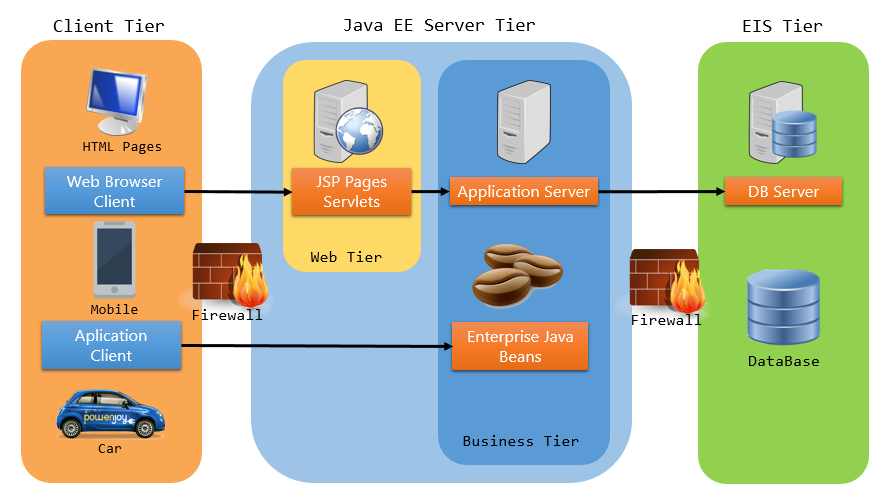
\includegraphics[width=1.2\textwidth]{ProposedSystemFW.png}}%
\caption {Proposed System Architecture}
\vspace*{0.5cm}
\end{figure}
\newpage

\subsection{High level components and their interaction}
Following our Architecture we organize the High level components on the 3 Tiers. This overview shows the interaction between the components and the entities they represent inside the System. Clients will have their User and CRM Components, distributed as Interfaces and Web Pages for the Apps. Inside the Server through Servlets and Session Beans a Session Manager will provide the services to the clients by communicating with the respective Controllers. Each Controller will manage and represent the System Entities previously explained in the RASD and will interface with a Persistent DataBase Connection to the DBMS. Helpers and Extra Feature Components are represented as well.

\begin{figure}[h]
\centering
\vspace*{\fill}
\noindent\makebox[\textwidth]{\includegraphics[width=1.35\textwidth]{HighLevelComponents.png}}%
\caption {High Level Component Structure}
\vspace*{0.5cm}
\end{figure}

\subsection{Component View}
\subsubsection{User Component}
Represents the User in the Client Tier that translates user actions and send requests to the Session Manager Component, then presents the output to the User. Is composed of several pages that present different types of information. Implement the Service Requests for each Actor, Web Pages in Web Server and Mobile Application and will have to interface with the central Server Component.
\subsubsection{CRM Component}
The CRM in the Client Tier will access just via browser, web server to the System. Is composed of a different set of pages and the Session Manager provides different services to it.
\begin{figure}[h]
\centering
\vspace*{\fill}
\noindent\makebox[\textwidth]{\includegraphics[width=0.5\textwidth]{UserCRMComponents.png}}%
\caption {Client Components}
\vspace*{0.5cm}
\end{figure}
\subsubsection{Car Component}
Represents the Car outside of our system that presents an interface to provide information and receive commands from the Car Controller Component.
\subsubsection{Reservation Controller}
Manages the Reservations made by Users, when a reservation is corfirmed, it will create the correspondant Ride.
\subsubsection{Ride Controller}
Manages the Active Rides. When a ride is finished, it creates a Payment using the Payment Controller.
\subsubsection{Payment Controller}
Implements the Logic to make a Payment or Transaction to a User Account, used by the Ride and the CRM Session Controllers.
\subsubsection{User Report Controller}
Used by the CRM Session to generate User Reports.
\begin{figure}[h]
\centering
\vspace*{\fill}
\noindent\makebox[\textwidth]{\includegraphics[width=0.8\textwidth]{ReservationRidePaymentComponents.png}}%
\caption {Entity Controllers}
\vspace*{0.5cm}
\end{figure}
\subsubsection{Session Manager}
The Session Manager is a Macro component. Will expose an API for User and CRM Clients. Will handle the main functionalities for them and will redirect requests to their respectve Controllers. Inside, the CRM and User Controllers will handle the CRM and User sessions respectively.
\newline
\begin{figure}[h]
\centering
\vspace*{\fill}
\noindent\makebox[\textwidth]{\includegraphics[width=0.87\textwidth]{SessionManagerComponent.png}}%
\caption {Session Manager}
\vspace*{0.5cm}
\end{figure}
\subsubsection{Car Controller}
Will manage Cars Status, Locations and interface to Cars to send them instructions.
\begin{figure}[h]
\centering
\vspace*{\fill}
\noindent\makebox[\textwidth]{\includegraphics[width=0.7\textwidth]{CarControllerComponent.png}}%
\caption {Car Controller}
\vspace*{0.5cm}
\end{figure}
\subsubsection{Location Helper}
Will provide an interface for Location queries. Can interface to an external Service Provider API (Google Maps).
\subsubsection{Chat Service}
 Will provide the chat platform to provide a channel of communication between Users and available CRMs
\subsubsection{Email Helper}
Will allow the System to communicate via mail with the Users (password, payment).
\newpage
\subsubsection{DBMS} 
Each Controller will implement a Persistent Entity for each class that will be mapped on the DB.
The Structure of the DB will mirror the Classes in our System.
\begin{figure}[h]
\centering
\vspace*{\fill}
\noindent\makebox[\textwidth]{\includegraphics[width=0.6\textwidth]{DatabaseStructure.png}}%
\caption {Database Structure}
\vspace*{0.5cm}
\end{figure}

\newpage
\subsection{Deployment View}
A first proposal for the Deployment View shows our main components in their deployed hardware as seen in the proposed Architechture. Mainly our Web, Application and DB Servers and the Client Devices. Our proposal for the communication protocols include:
\begin{itemize} 
\item The Web Clients communicate to the Web Server via HTTPS. 
\item The Application Server exposes a RESTful API for the Web Server, Mobile Apps and Cars. 
\item The Application Server communicates with the DB Server using JDBC connection.
\end{itemize}
\begin{figure}[h]
\centering
\vspace*{\fill}
\noindent\makebox[\textwidth]{\includegraphics[width=1.2\textwidth]{DeploymentView.png}}%
\caption {Deployment View}
\vspace*{0.5cm}
\end{figure}
\newpage

\subsection{Runtime View}
\subsection{Component Interfaces}
\subsection{Selected Architectural Styles and Patterns}
\subsection{Other Design Decisions}

\section{Algorithm Design}

\section{User Interface Design}
For our User Interface (UI) we'll offer a mobile App for Users and a desktop web App for Users and CRM. They will offer:
\begin {itemize}
\item \textbf{LogIn Page:} First screen of the app with the LogIn and SignIn options.
\begin{figure}[h]
\centering
\vspace*{\fill}
\noindent\makebox[\textwidth]{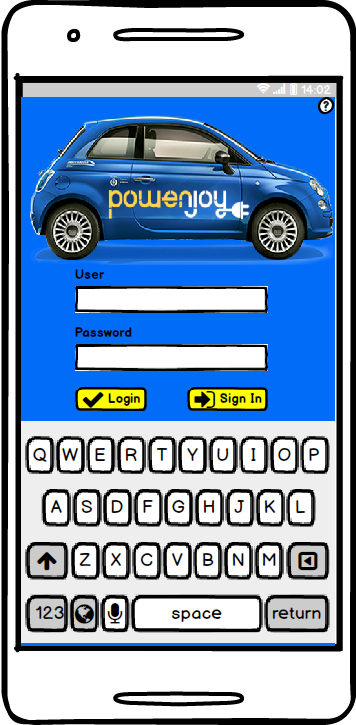
\includegraphics[width=0.28\textwidth]{1.png}}%
\caption {UI LogIn Page}
\vspace*{0.2cm}
\end{figure}
\pagebreak
\item \textbf{Main Page:} Main page of the app where the user sees the map his location and selects the available cars. In Case of CRM, it can see all Cars.
\begin{figure}[h]
\centering
\vspace*{\fill}
\noindent\makebox[\textwidth]{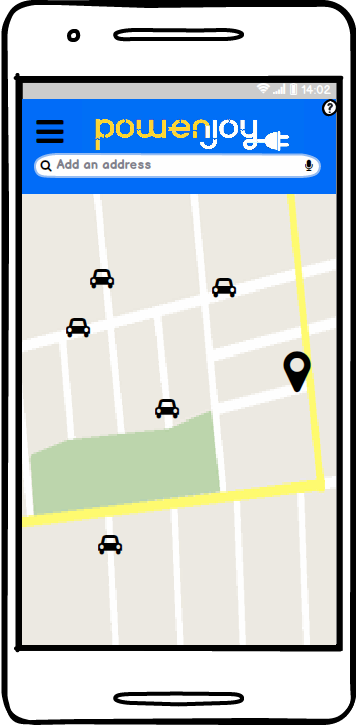
\includegraphics[width=0.28\textwidth]{2.png}}%
\caption {UI Main Page}
\vspace*{0.2cm}
\end{figure}
\item \textbf{Car Details Page:} Once a Car is selected this page allows to reserve a car and contais informations for the decision.
\begin{figure}[h!]
\centering
\vspace*{\fill}
\noindent\makebox[\textwidth]{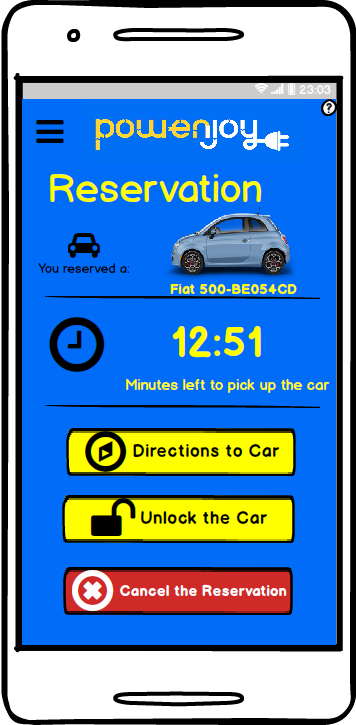
\includegraphics[width=0.28\textwidth]{4.png}}%
\caption {UI Car Details Page}
\vspace*{0.2cm}
\end{figure}
\pagebreak
\item \textbf{Reservation Page:} Once the Reservation is made, the User can see the details of her/his Reservation and have the option to cancel it.
\begin{figure}[h!]
\centering
\vspace*{\fill}
\noindent\makebox[\textwidth]{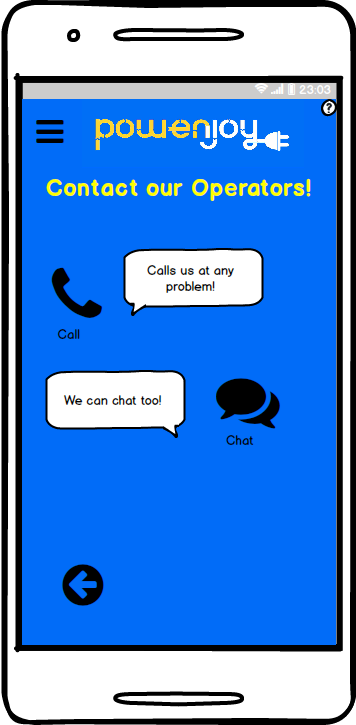
\includegraphics[width=0.28\textwidth]{5.png}}%
\caption {UI Reservation Page}
\vspace*{0.2cm}
\end{figure}
\item \textbf{Ride Page:} Once a Ride started this page shows the details of the current ride, it's present also in the Car screen App.
\begin{figure}[h!]
\centering
\vspace*{\fill}
\noindent\makebox[\textwidth]{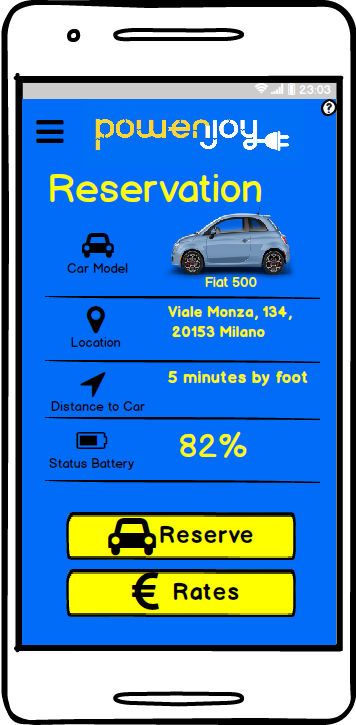
\includegraphics[width=0.36\textwidth]{3.png}}%
\caption {UI Mobile Ride Page}
\vspace*{0.2cm}
\end{figure}
\pagebreak
\begin{figure}[h!]
\centering
\vspace*{\fill}
\noindent\makebox[\textwidth]{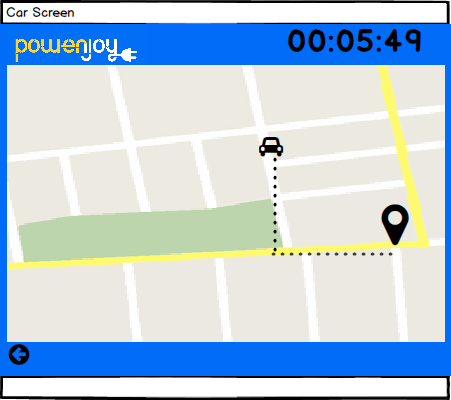
\includegraphics[width=0.7\textwidth]{CarScreen.png}}%
\caption {UI Car Ride Page.}
\vspace*{0.2cm}
\end{figure}
\item \textbf{Email Page:} While not part of the App UI, the System should respond with an email to the User at the end of the Ride showing the final details for it.
\begin{figure}[h!]
\centering
\vspace*{\fill}
\noindent\makebox[\textwidth]{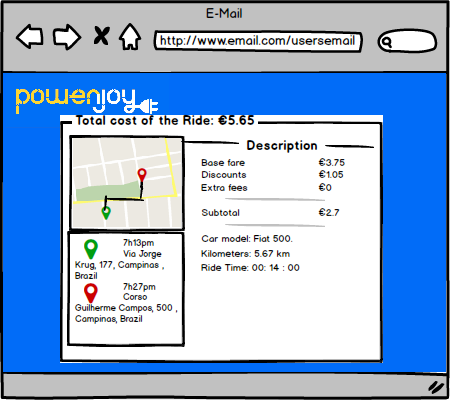
\includegraphics[width=0.7\textwidth]{EmailUser.png}}%
\caption {UI Email Page}
\vspace*{0.2cm}
\end{figure}
\pagebreak
\item \textbf{Contact Page:} Page where the User can contact the CRM operator.
\begin{figure}[h!]
\centering
\vspace*{\fill}
\noindent\makebox[\textwidth]{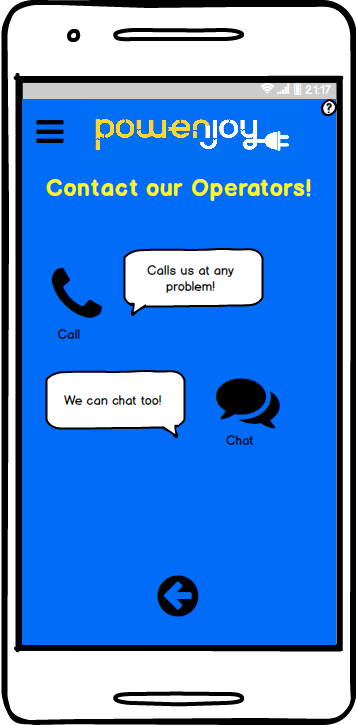
\includegraphics[width=0.28\textwidth]{6.png}}%
\caption {UI Contact Page}
\vspace*{0.2cm}
\end{figure}
\end{itemize}

\section{Requirements Traceability}
\section{Effort Spent}
\begin{tabular}{ | l | l | l | l | }
\hline
	\textbf {Date} & \textbf {Domenico} & \textbf {Caio} & \textbf {Matheus} \\ \hline
	27/11/16& 1h & 1h & 1h  \\ \hline
	28/11/16& 2h & - & - \\ \hline
	29/11/16& 2h & - & - \\ \hline
	30/11/16& 3h & - & - \\ \hline
	31/11/16& 1h & - & - \\ \hline
	01/12/16& - & 1h & - \\ \hline
	02/12/16& 5h & 2h & - \\ \hline
	03/12/16& 2h & 4h & - \\ \hline
	04/12/16& - & - & - \\ \hline
	05/12/16& - & - & - \\ \hline
	06/12/16& - & - & - \\ \hline
	07/12/16& - & - & - \\ \hline
	08/12/16& - & - & - \\ \hline
	09/12/16& - & - & - \\ \hline
	10/12/16& - & - & - \\ \hline
	11/12/16& - & - & - \\ \hline
\end{tabular}
\newpage

\section{References}
\newpage


\section{Used Tools}
Keeping track of the Tools used during develop the DD document were:
\begin{itemize}
	\item \textbf{GitHub:} for Version Control
	\item \textbf {Dia Diagram Editor:} for UML Diagrams
	\item \textbf {TeXworks:} for LaTex editing of this Document
\end{itemize}
\newpage

\section{Changelog}
As the project and design decisions may change during the development this document is also prone to change.
We'll document every version in this part.
\begin{itemize}
\item \textbf {Version 1.1:} 11/12/2016
\end{itemize}
\end{document}
